%% document class
\documentclass[14pt, a4paper]{extreport}

%% packages 

\usepackage{graphicx} % needed for \includegraphics (images)
\usepackage{blindtext} % needed for createing dummy text packages
\usepackage{arabtex} % needed if we write some arabic text
\usepackage{utf8}
\usepackage{times}  % or 'times' package for Times New Roman font
\usepackage{setspace}    % For setting line spacing
\usepackage[hidelinks]{hyperref} % support for hyperlinks
\usepackage{enumitem}  % for changing label of enumrate
\usepackage{tabularx} % in the preamble
\usepackage{array}  
\usepackage[export]{adjustbox} % graphicx is also included


%% page settings 
%% page settings

%\usepackage{wordlike}
\usepackage[top=2cm, bottom=1.8cm, left=2.5cm, right=2.5cm]{geometry} % needed for page border settings
\usepackage{fancyhdr} % needed for head and foot options
\setcode{utf8}

% Set the depth of the table of contents
\setcounter{tocdepth}{2}




%% own commands 
\newcommand{\tbi}[1]{\textbf{\textit{#1}}}
\newcommand{\customitem}[1]{\item \textbf{#1} \hfill}

%--------------------------------------------------------
\begin{document}

\begin{titlepage} 
	\newcommand{\HRule}{\rule{\linewidth}{0.5mm}} % Defines a new command for horizontal lines, change thickness here
	
	\begin{center}
		\begin{minipage}{0.15\textwidth}%
			
\includegraphics[width=2.2cm]{content/Logo copy.png}
		\end{minipage}
		\begin{minipage}{0.69\textwidth}%
			\center
			\textsc{\large  Computer And Artificial Intelligence}\\[0.5cm]
			\textsc{\normalsize Graduation Project}\\[0.5cm]
		\end{minipage}\hfill
		\begin{minipage}{0.15\textwidth}%
			
\includegraphics[width=2.2cm]{content/faculty.png}
        \end{minipage}
	\end{center}

	\center % Centre everything on the page
	
	%------------------------------------------------
	%	Title
	%------------------------------------------------
	\vspace{3cm}
	\HRule\\[0.4cm]
	
	{\huge\bfseries NeuraLearn Academy}\\[0.4cm] % Title of your document
	
	\HRule\\[1.5cm]
	
	%------------------------------------------------
	%	Author(s)
	%------------------------------------------------
	\begin{spacing}{1}
		\begin{center}
			\large
			Khaled Mohamad Fathy \\
			Sherif Ahmed Shehata Hammam \\
			Mahmoud Ahmad Zitony \\
			Basem Yahia Abdelatif Ahmed \\ 
			Karim abdelazim Mohamed shehtata \\
			Mohamed Ashraf Mohamed Badwy \\ 
			Beshoy Tag Makram \\
			\vspace{50mm}
		\end{center}
	\end{spacing}

	\begin{minipage}{\textwidth}
		\begin{center}
			\large
			\textit{Supervisor}\\
			Dr. Gehad \textsc{hassan}
		\end{center}
	\end{minipage}
	
	%------------------------------------------------
	%	Date
	%------------------------------------------------
	
	\vfill\vfill\vfill % Position the date 3/4 down the remaining page
	
	{\large\today} % Date, change the \today to a set date if you want to be precise
	
	\vfill % Push the date up 1/4 of the remaining page
	
\end{titlepage}

\pagestyle{plain}

\begin{abstract}
NeuraLearnAcademy - Revolutionizing Distance Learning with AI-Enhanced Tools

In response to the persistent challenges faced by learners in online education platforms, 
NeuraLearnAcademy emerges as an innovative solution, pioneering a paradigm 
shift in the landscape of distance learning.

This electronic platform harnesses the power of advanced technologies, specifically Large Language Model (LLM) and Machine Learning (ML), to address and overcome
the limitations inherent in existing online learning environments. It introduces a suite of tools and features meticulously designed to enhance the learning experience.

The platform tackles the issues of low engagement through interactive elements
such as quizzes and discussions. It addresses the inadequacies of assessment methods by incorporating a range of evaluation techniques, ensuring a comprehensive understanding of the course material.
\end{abstract}
    
\renewcommand{\abstractname}{Acknowledgements}
\begin{abstract}
    We would like to take this opportunity to express our sincere
    appreciation and best wishes to our devoted supervisor, Dr. Jehad,
    for her great leadership and ongoing motivation during the completion of
    this project. The assistance, and guidance she occasionally provided will
    help us get far along in the life's journey we are about to take.

    We also take this occasion to thank Faculty of Computers and
    Artificial Intelligence Council for their support and work in getting us all
    the resources we need.

    We would especially like to thank the FCAI members for the useful
    information they gave in their respective domains.
    Finally, we express our gratitude to Almighty, our parents, and
    everyone who has provided assistance, encouragement, and support.
\end{abstract}

    

\tableofcontents 
\listoffigures  


\chapter{Introduction}

\section{Introduction}


\subsection{Problem Definition}

Over the past decade, online learning has experienced significant growth, capitalizing on the fusion of the internet and education to offer individuals the opportunity to acquire new skills. The COVID-19 pandemic has further propelled online learning into a central position in people's lives, compelling educational institutions and businesses to embrace remote work and education. This surge in demand has given rise to a multitude of online learning platforms like Udemy, Coursera, Lynda, Skillshare, and Udacity, serving millions of users and evolving based on different user needs. Additionally, prestigious universities such as Stanford and Harvard are contributing to the democratization of education by providing accessible online courses spanning computer science, engineering, mathematics, business, art, and personal development.

\subsubsection*{Advantages of Online Learning}

\begin{itemize}[label=--]
	\item \textbf{Efficiency}: Online learning enables teachers to efficiently deliver lessons using tools such as videos and PDFs.
	\item \textbf{Accessibility of Time and Place}: Students can attend classes from any location, breaking geographical barriers and reaching a broader network of students.
	\item \textbf{Affordability}: Online education proves to be more cost-effective compared to traditional learning methods.
	\item \textbf{Suits a Variety of Learning Styles}: Online learning caters to diverse learning styles, accommodating visual, auditory, and independent learners.
\end{itemize}

\subsubsection*{Disadvantages of Online Learning}

\begin{itemize}[label=--]
	\item \textbf{Lack of Personal Interaction}: Online learning lacks face-to-face interaction between students and instructors, missing the dynamic of traditional classrooms.
	\item \textbf{Limited Hands-On Experience}: Certain disciplines require hands-on experience, which online learning may struggle to provide adequately.
	\item \textbf{Interactivity}: While online education offers interactive elements like discussion forums and virtual classrooms, the level of engagement may vary.
	\item \textbf{Assessment Methods}: Digital assessments in online education may be convenient, but traditional education often incorporates a mix of digital and traditional assessment methods.
\end{itemize}

\subsection{The Role of Generative AI}

Generative Artificial Intelligence (AI) has become a revolutionary force in education, particularly in online learning. Harnessing the advancements in technology, educators are leveraging generative AI to create personalized, engaging experiences for students. In this article, we will explore how generative AI transforms student interaction with online materials, fostering a more dynamic and effective learning environment.

\section{Introducing NeuraLearnAcademy}

The project aims to develop a new generation of learning platforms that address the challenges of online learning using Generative AI. NeuraLearnAcademy merges the power of Generative AI with an online platform, offering a solution to the drawbacks associated with traditional online education. This innovative approach aims to enhance interactivity, overcome the lack of personal interaction, and provide a more immersive and effective learning experience for students.

\subsection{Problem Solution}

Generative Artificial Intelligence (Generative AI) refers to a subset of artificial intelligence that focuses on creating and generating new content, such as images, text, or other data types. Unlike traditional AI models that rely on pre-existing data for classification or prediction tasks, generative models have the capability to generate novel and coherent output. These models learn patterns and structures from training data and use that knowledge to create new, similar content.

A language model is a type of artificial intelligence that is specifically designed to understand and generate human-like language. Language models learn the structure, grammar, and context of language from large datasets and can be utilized for various natural language processing tasks, such as machine translation, text summarization, and text completion. One notable example of a language model is OpenAI's GPT (Generative Pre-trained Transformer), which has demonstrated remarkable proficiency in understanding and generating coherent text.

\section{Generating Questions and Summarizing Video Transcripts}

Transcribing videos and extracting valuable information from them can be a powerful method for knowledge extraction. This process can be further enhanced by utilizing language model techniques for generating questions and summarizing the content.

Once you have identified key information from the transcripts, you can use language models to generate questions automatically. These questions can be crafted based on the content, aiming to cover essential topics, clarify ambiguities, or prompt further exploration. Question generation models can be trained on existing datasets or fine-tuned for specific domains. There are various approaches to summarizing textual content, and they can be adapted to video transcripts as well. Extractive summarization involves selecting the most important sentences or phrases from the transcript, while abstractive summarization generates a concise summary in the model's own words.

\section{Integration with Platform}

Integrate the trained question-answering model seamlessly into your educational platform. Design a user-friendly interface that allows users to submit their questions or feedback related to the video content. Enable the question-answer model to generate dynamic responses based on the context of the questions and feedback. The model should consider the entire transcript, relevant sections, and any additional information available to provide accurate and context-aware responses.

Implement interactive platforms or chatbots that can engage with users based on the generated questions. These platforms can provide a more dynamic and personalized learning experience.

\section{Motivation}

In today's education scene, Machine Learning isn't just a passing trend; it is a powerful tool that can fundamentally transform the way we teach and learn. By integrating Machine Learning into our project, we want to use its capabilities to revolutionize traditional educational methods and improve the overall learning experience.

\subsection{Comprehensive Understanding}

\begin{itemize}[label=--]
	\item \textbf{Goal}: Ensure every student comprehensively understands each chapter of the course.
	\item \textbf{How}: Implement a post-chapter feedback mechanism where students interact with ChatGPT, expressing what they've grasped and clarifying any uncertainties. This iterative process ensures a solid foundation before progressing to subsequent chapters.
\end{itemize}

\subsection{Personalized Knowledge Assessment}

\begin{itemize}[label=--]
	\item \textbf{Goal}: Tailor assessments to each student's understanding and learning pace.
	\item \textbf{How}: Develop a dynamic quiz model that adapts to individual progress, assessing not only factual knowledge but also the ability to connect concepts across chapters. This personalized approach enhances the learning experience and identifies areas that may need additional focus.
\end{itemize}

\subsection{Summarization for Reinforcement}

\begin{itemize}[label=--]
	\item \textbf{Goal}: Reinforce learning through concise summarization.
	\item \textbf{How}: Implement a summarization model that extracts key points from each chapter, generating a PDF file containing both a textual summary and a visual representation of important concepts discussed in the video. This resource aids in reinforcement and serves as a quick reference for students.
\end{itemize}

\subsection{Iterative Learning Journey}

\begin{itemize}[label=--]
	\item \textbf{Goal}: Facilitate a structured and iterative learning journey.
	\item \textbf{How}: Restructure the course format to unlock subsequent chapters only after the student submits an understanding summary for the previous chapter. This ensures a stepwise progression, solidifying knowledge before advancing.
\end{itemize}

\subsection{Continuous Improvement Feedback Loop}

\begin{itemize}[label=--]
	\item \textbf{Goal}: Establish a continuous improvement feedback loop.
	\item \textbf{How}: Gather feedback from students on the effectiveness of the ChatGPT interactions, summarization model, and quizzes. Utilize this feedback to enhance the platform, ensuring its responsiveness to the diverse needs and learning styles of users.
\end{itemize}

By aligning these goals and objectives, NeuraLearnAcademy aims to create a dynamic and adaptive learning environment that not only imparts knowledge but also actively engages students in the learning process, fostering a deeper and more sustained understanding of course material.

\section{Project Limitations}

The primary limitation lies in the accuracy of assessing students to gauge their comprehension of specific course sections. Ensuring precise evaluation of understanding within the platform is a critical focus, recognizing potential challenges in achieving absolute accuracy due to inherent complexities in subjective assessments.



\chapter{Project Planning}

\section{Why Planning ?}
In project management, planning is crucial for successful project implementation. so we should carefully planning and choose the methodology that fit our project and specify, prioritize, manage the main project tasks, as well as identify and manage potential risks.
Furthermore, effective planning can significantly enhance project performance and success rates, leading to cost and time savings. Additionally, it improves team communication, ensuring the best utilization of resources making it easier to track project goals and outcomes.

\section{Scrum Overview}
What is Scrum? Scrum is an agile way to manage work. Ever few weeks (typically two to four), teams deliver a fully functional chunk of work (an increment). Teams and the business use the feedback from each delivery to determine what to build next, or how to adapt what they've already built.
Scrum works through a series of events that happen over a defined period of time: that time period is called a sprint. Sprints are short timeboxes during which the team turns ideas into working product. The events then repeat every sprint.
\begin{figure}[h!]
	\centering
	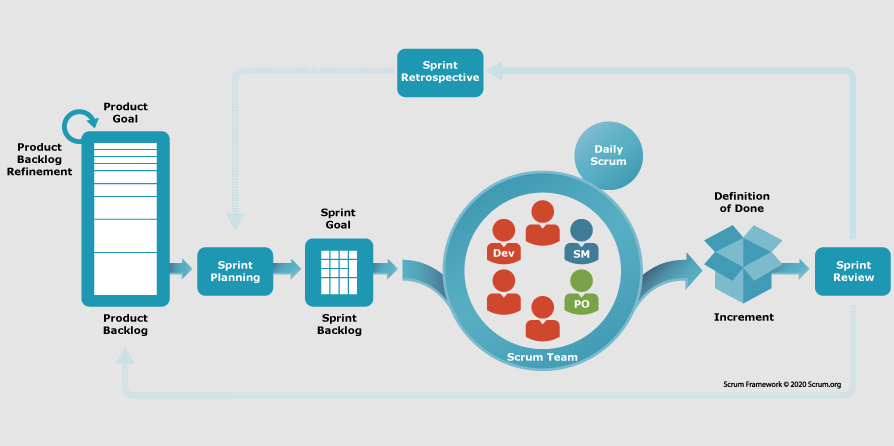
\includegraphics[width=\textwidth, height=4cm]{figures/scrum-overview.png}
	\caption{Scrum Overview}
\end{figure}


\newpage 

\section{Scrum Activities and Events}
\begin{itemize}
	\item \textbf{Sprint Planning.}  \hfill \vspace{0.2cm} \\
	Each sprint begins with a sprint planning meeting, where the team leader presents the top items on the product backlog to the team, and team members figure out how much work they can commit to during the coming sprint.
	
	\item \textbf{The Sprint.} \hfill \vspace{0.2cm} \\
	During each sprint, the team takes a small set of features from idea to fully implemented and tested functionality. At the end, these features are done and could potentially be released.
	
	\item \textbf{Daily Scrum.} \hfill \vspace{0.2cm} \\
	On each day of the sprint, all team members attend a daily scrum meeting. Daily scrums are a way for team members to synchronize their work and collaborate to move that work to done. The daily meetings last no more than 15 minutes and are intended to give the team a time to share what they worked on the prior day, will work on that day, and identify any impediments to progress.
	
	\item  \textbf{Sprint Review.}  \hfill \vspace{0.2cm} \\
	At the end of a sprint, the team conducts a sprint review during which the team demonstrates the new functionality to the stakeholder who wishes to provide feedback that could influence the next sprint. It's critical that the sprint review remains informal and doesn't become its own task, distracting from the work itself.
\end{itemize}

\section{Why Scrum?}
\begin{enumerate}
	\item \textbf{Responsive team:} 
	with scrum, our teams will be more responsive in their productivity, especially as changes and pivots are required. The scrum discipline requires frequent reviewing of progress, which often demands changes to prevent a project from failing.
	
	\item \textbf{More accurate planning:}
	by using Scrum, our plans will be less apt to fail. Why? Because our teams are constantly putting in the effort to keep them on track by shifting and changing as needed. And because of the way scrum is designed, our teams will constantly be reflecting how things are going and can make small or large adjustments to the plans, according to the winds of change. By adhering to scrum artifacts and events, our plans are far less likely to fail.
	
	\item \textbf{Everyone in sync:}
	when using scrum, a project’s stakeholders are always in sync. And because the scrum methodology prioritizes individuals and interactions over all else, keeping everyone involved in sync is actually built into the process.
	
	\item \textbf{Flexible priorities:}
	with scrum, it’s very easy to prioritize and re-prioritize as the project moves through the process. With this ability, our developer team become more flexible and our project becomes more agile. This also makes it possible to easily (and quickly) adjust short-term goals while still adhering to the overall strategy of the project.
	
	\item \textbf{More control:}
	finally, we will have more control over the entire project. That’s not to say we will be able to better control our staff. No. Instead, we have more control over the direction and flow of the development process. And when we have consistent input from developers and other stakeholders, it lends a level of cohesion to the process you wouldn’t otherwise have.
\end{enumerate}

\section{Main tasks of our project}
\begin{itemize}
    \item Design UI and UX
    \item Design database diagrams
    \item Implement the frontend
    \item Implement the backend
    \item Test and debug the project
    \item Writing the documentation
\end{itemize}

\newpage

\begin{figure}[h!]
	\centering
	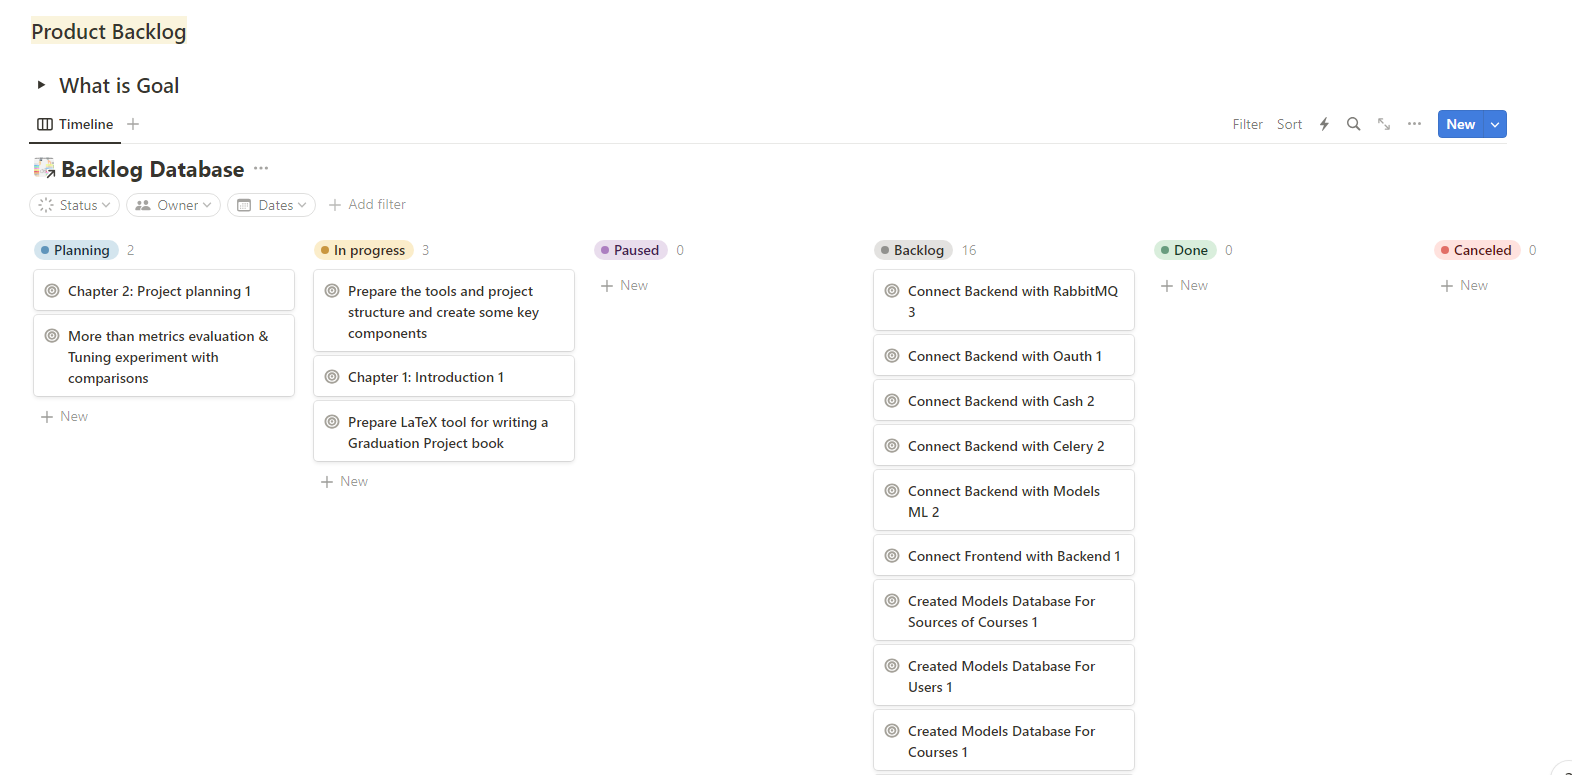
\includegraphics[width=0.95\textwidth]{figures/snapshot-of-backlog-database.png}
	\caption{Snapshot Of backlog}
\end{figure}

\begin{figure}[h!]
	\centering
	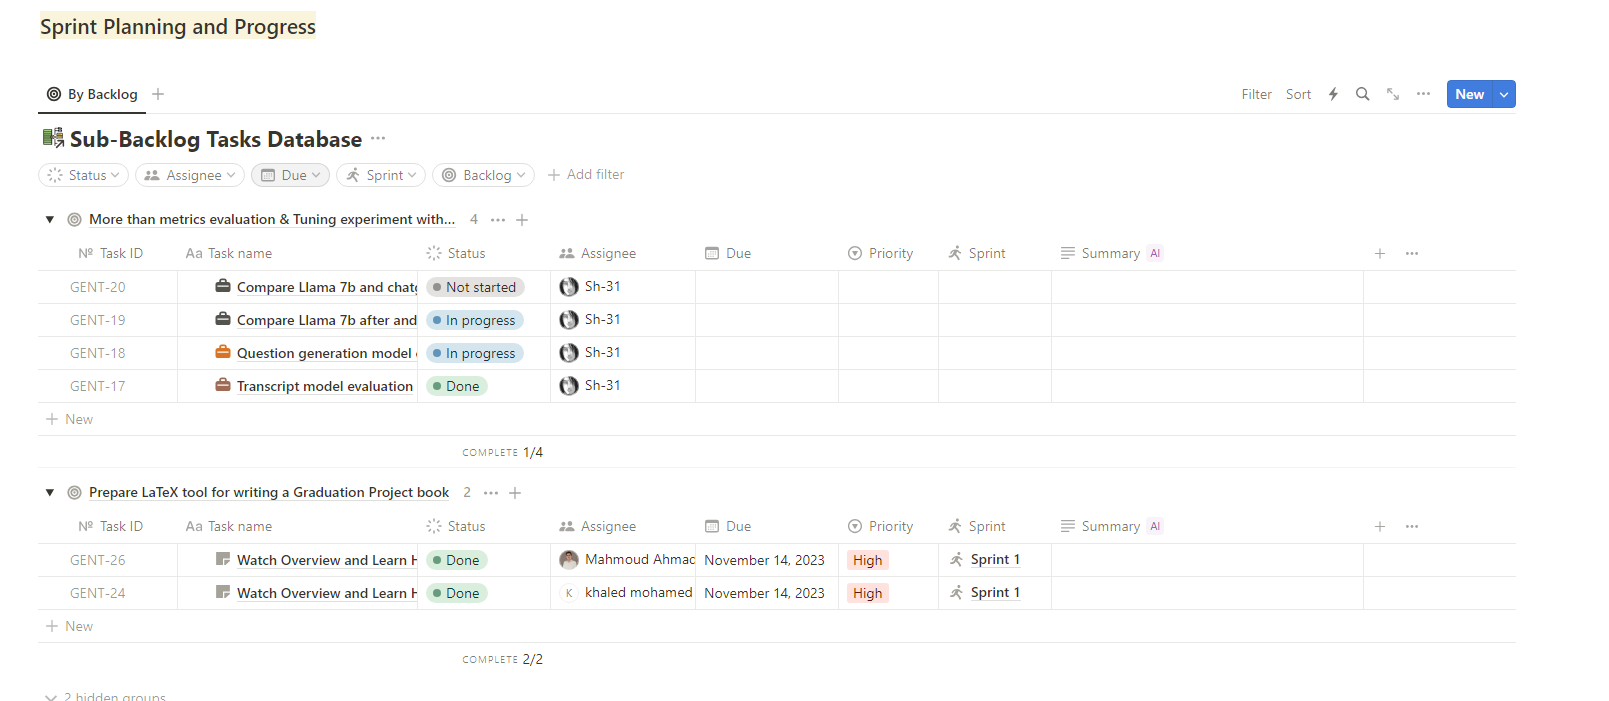
\includegraphics[width=0.95\textwidth]{figures/snapshot-of-sprint-planning.png}
	\caption{Snapshot Of sprint planning}
\end{figure}

\newpage 

\section{Risk Identification}
Project Risk Management includes the processes of conducting 
risk management planning, identification, analysis, response 
planning, and controlling risk on a project. The objectives 
of project risk management are to increase the likelihood and 
impact of positive events and decrease the likelihood and impact 
of negative events in the project. The key step in risk management
planning is project risk identification. Risk identification
identifies the risks that could have an impact on the project 
and lists their characteristics. However, as recommended, we should
avoid devoting too much time to risk identification.

\subsection{Technology Dependencies}
\textbf{Risk:} Dependencies on third-party technologies or frameworks may undergo updates or discontinuation, impacting the platform's functionality. \\
\textbf{Mitigation:} Regularly update and maintain dependencies, conduct thorough compatibility checks, and have contingency plans for potential disruptions.

\subsection{Data Security and Privacy}
\textbf{Risk:} Security breaches or data privacy issues could compromise user information and erode trust. \\
\textbf{Mitigation:} Implement robust security measures, adhere to data protection regulations, and conduct regular security audits to identify and address vulnerabilities.

\subsection{User Adoption}
\textbf{Risk:} Users may find the platform challenging to navigate, leading to low adoption rates. \\
\textbf{Mitigation:} Implement a user-friendly onboarding process, provide clear documentation, and offer responsive customer support to ensure users can easily navigate and utilize the platform.

\newpage 

\subsection{Scalability Challenges}
\textbf{Risk:} An unexpected surge in user traffic may lead to server overload, causing system slowdowns or crashes. \\
\textbf{Mitigation:} Utilize scalable cloud services, conduct load testing, and have a scalable infrastructure in place to accommodate a growing user base.

\subsection{Content Quality}
\textbf{Risk:} Inaccuracies or insufficient quality in course content may impact the effectiveness of the learning experience. \\
\textbf{Mitigation:} Establish a thorough content review process, actively seek user feedback on content quality, and iterate based on user input.

\subsection{Technological Obsolescence}
\textbf{Risk:} Rapid advancements in technology may render certain components of the platform obsolete. \\
\textbf{Mitigation:} Regularly update the technological stack, monitor emerging technologies, and plan for phased upgrades to avoid obsolescence.

\subsection{Adaptability to Learning Styles}
\textbf{Risk:} The platform may not fully cater to the diverse learning styles and preferences of users. \\
\textbf{Mitigation:} Gather user feedback on learning experiences, conduct usability testing with a diverse user base, and iterate the platform design to enhance adaptability.

\subsection{Integration with External Systems}
\textbf{Risk:} Challenges in integrating seamlessly with external platforms or tools may hinder collaboration opportunities. \\
\textbf{Mitigation:} Conduct thorough compatibility testing with external systems, establish robust APIs, and foster collaborations through ongoing communication with potential partners.

\newpage 

\subsection{Regulatory Compliance}
\textbf{Risk:} Changes in educational or data protection regulations may necessitate adjustments to the platform. \\
\textbf{Mitigation:} Stay informed about regulatory changes, conduct regular compliance checks, and adapt the platform accordingly to ensure alignment with current standards.

\subsection{User Technical Proficiency}
\textbf{Risk:} Users with limited technological skills may struggle to navigate and utilize the platform effectively. \\
\textbf{Mitigation:} Provide comprehensive user guides, tutorials, and responsive customer support to assist users with varying levels of technical proficiency.



\chapter{System Analysis}

\section{System Requirements}
A requirement is simply a statement of what the system must do or what characteristics
it needs to have. During a systems development project, requirements will be created
that describe what the business needs (business requirements), what the users
need to do (user requirements), what the software should do (functional requirements),
characteristics the system should have (nonfunctional requirements), and how
the system should be built (system requirements).

\subsection{Functional Requirements}
Functional requirements are the specifications of the product’s functions
(features). In another words, functional requirements define what precisely a
software must do and how the system must respond to inputs. Functional
requirements define the software's goals, meaning that the software will not work if
these requirements are not met.

\begin{enumerate}
    \customitem{Authentication}
        \begin{enumerate}[label*=\arabic*.]
            \item The system will allow users to create an account.
            \item The system must validate users credentials to login.
            \item Users should have the ability to reset their passwords in case of forgotten credentials. 
        \end{enumerate}
    \customitem{Enroll Courses}
        \begin{enumerate}[label*=\arabic*.]
            \item Students can enroll courses and see course content
              We will extend this to enroll paid course wit credit card, debit card etc. in the future.
        \end{enumerate}
    \item \textbf{Course Managment} \hfill
        \begin{enumerate}[label*=\arabic*.]
            \item Instructors can create a course and upload to our website.
            \item Instructors can upload various types of course content, including text, multimedia, and documents.
            \item Only authorized instructors should have the ability to modify or update course content.
        \end{enumerate}
\end{enumerate}

\subsection{Non-Functional Requirements}
Non-functional Requirements define system attributes such as security,
reliability, performance, maintainability, scalability, and usability. They serve as
constraints or restrictions on the design of the system across the different backlogs.
Also known as system qualities, non-functional requirements are just as critical as
functional requirements. They ensure the usability and effectiveness of the entire
system. They specify criteria that judge the operation of a system, rather than specific
behaviors.

\begin{itemize}
    \customitem{Performance} \vspace{0.2cm} \\
        The application should be able to handle large numbers of concurrent users.  
    \customitem{Security} \vspace{0.2cm} \\
        The application should protect user data from
        unauthorized access or theft.
    \customitem{Scalability} \vspace{0.2cm} \\
        The application should be able to handle an increasing number of users and services.
    \customitem{User-friendliness} \vspace{0.2cm} \\
        The application should be easy to use and navigate, with
        clear instructions and explanations of the analysis process.
    \customitem{Privacy} \vspace{0.2cm} \\
        The application should have a clear privacy policy and
        should not retain user data
    
\end{itemize}

\newpage

\section{Exploring Trade-offs Architectures}
\begin{itemize}
    \item Sequence to sequence models (LSTM-GRU-RNN):
    \begin{itemize}
        \item Difficulty in Incorporating Domain Knowledge 
        \item Limited Interpretability
        \item Handling Varied Output Lengths
    \end{itemize}
    \item Encoder-Decoder Transformer:
    \begin{itemize}
        \item Transformer architecture, with self-attention mechanisms, has been widely used in Seq2Seq tasks.
        \item It does come with some potential disadvantages, including high training costs.
        \item Alternative way Fine-Tuning and Transfer Learning.
    \end{itemize}
\end{itemize}

\begin{figure}[h!]
	\centering
	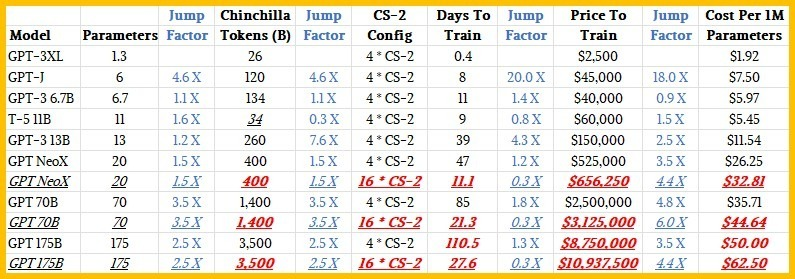
\includegraphics[max height=\textheight,max width=\textwidth]{figures/transformer.jpeg}
	\caption{Transformer}
\end{figure}
% \section{Proposed Model}

\begin{figure}[h!]
	\centering
	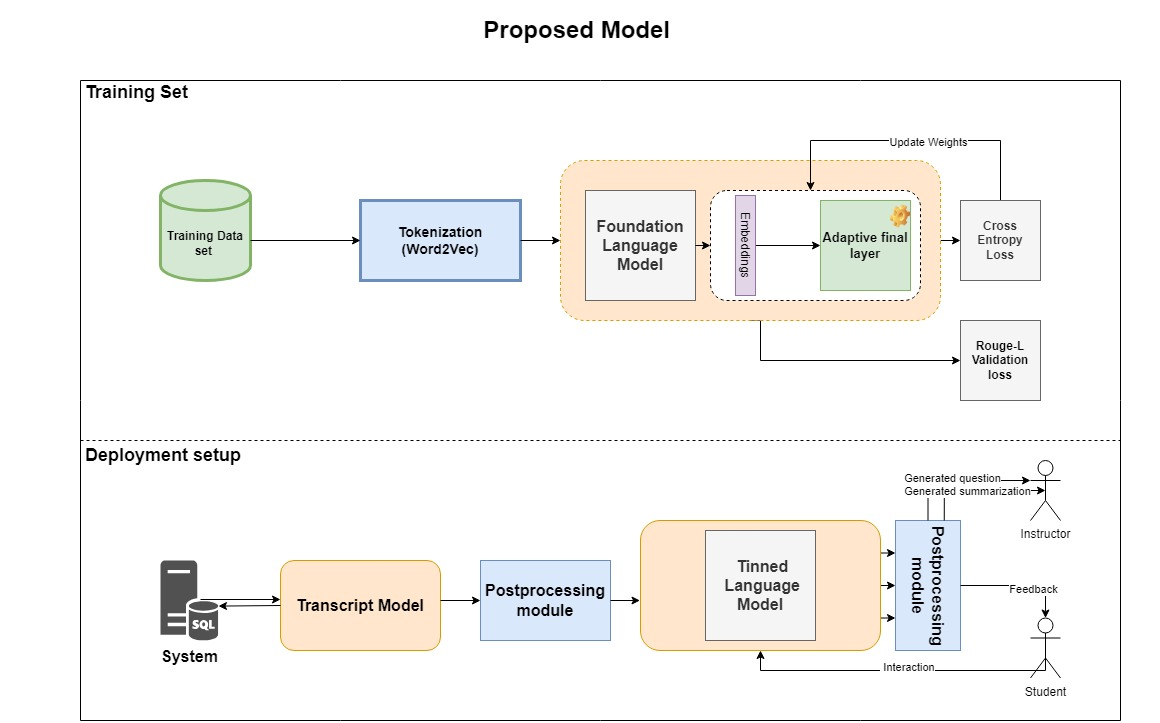
\includegraphics[max height=\textheight,max width=\textwidth]{figures/proposal-model.jpeg}
	\caption{Proposed Model}
\end{figure}

\newpage
\noindent
The motivation behind designing a large language model with adaptive layers lies in the pursuit of creating a model that can efficiently and effectively adapt to the complexities and nuances of different datasets and tasks

\subsection{Flexibility Across Diverse Tasks:}

Adaptive layers enhance the model's flexibility to handle various natural language processing tasks. Whether it's text classification, language translation, sentiment analysis, or any other task, the adaptive layers allow the model to dynamically adjust its parameters based on the specific requirements of each task.

\subsection{Optimizing for Different Data Distributions:}

Different datasets may exhibit varying data distributions and characteristics. Adaptive layers provide a mechanism for the model to adapt its learning rates or normalization parameters dynamically, optimizing its performance for the specific patterns present in the data.



\subsection{Enhanced Convergence and Training Speed:}

Adaptive learning rate methods contribute to faster convergence during training. By adapting learning rates for individual parameters, the model can converge more quickly, leading to reduced training times and improved overall efficiency.
\section{Use Case Analysis}
A Use Case is a type of behavioral representation that shows the interactions
between a system and its users, or actors. It is used to represent and model the
functionality of a system. The main purpose of a use case diagram is to capture
the functional requirements of a system. 
\\ \\ \\
\textbf{There are two formats to represent use cases:}
\begin{enumerate}
    \item Use case diagram.
    \item Use case specifications or scenario in textual format.
\end{enumerate}

\newpage

\section{Use Case Diagram}
\begin{figure}[h!]
	\centering
	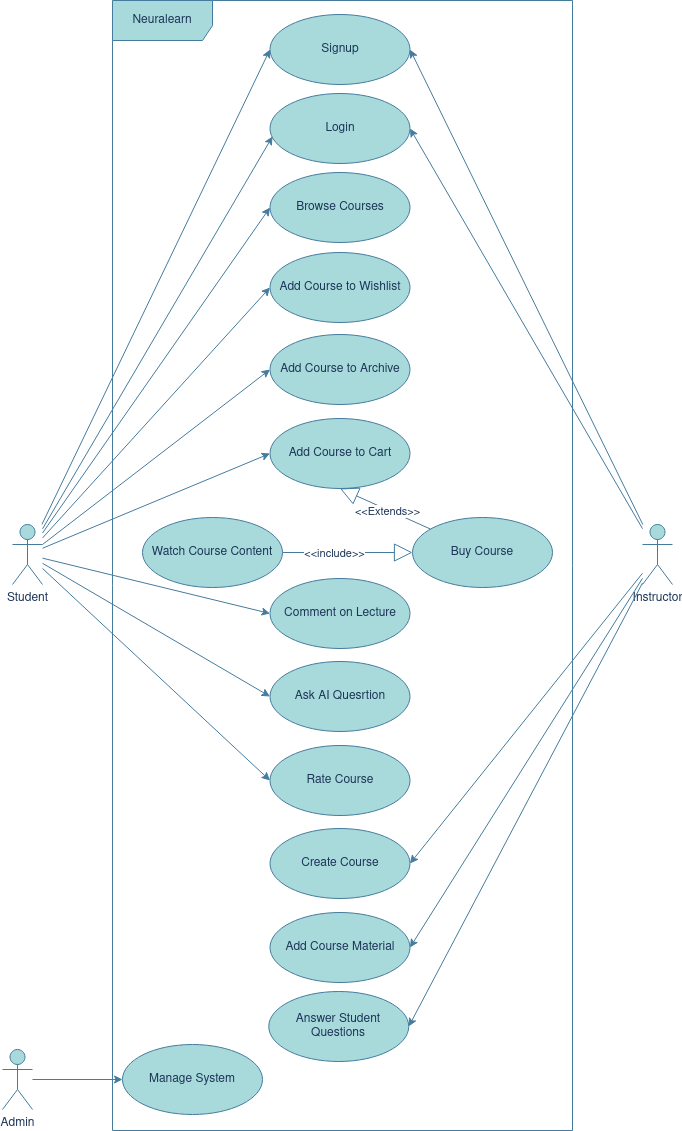
\includegraphics[scale=0.5]{figures/UML-Use-Case.png}
	\caption{UML Use Case Diagram}
\end{figure}

\newpage

\begin{table}[h!]
    \centering
    \caption{Use Case: Sign-Up}
    \bgroup
    \def\arraystretch{1.5}%  1 is the default, change whatever you need
    \begin{tabular}{|m{4cm}|m{11cm}|}
        \hline
        \textbf{Use Case Name} & Sign-Up \\
        \hline
        \textbf{Number} & 1 \\
        \hline
        \textbf{Actor} & Student, Instructor, and Admin \\
        \hline
        \textbf{Preconditions} & 
        \begin{itemize}[noitemsep,topsep=0pt] % Adjust the value as needed
            \item Full name
            \item Email address
            \item Date of birth
            \item Username
            \item Password (and password confirmation)
        \end{itemize} \\
        \hline
        \textbf{Flow of Events} & 
        \begin{itemize}[noitemsep,topsep=0pt]
            \item The student clicks on the sign-up button, leading to the registration form page.
            \item The form prompts the student to enter their full name, email address, date of birth, username, and password.
            \item The student fills in the required information and clicks the "Submit" button.
        \end{itemize} \\
        \hline
        \textbf{Exception} & 
        If the verification email is not received, the student may have the option to request a new verification. \\
        \hline
    \end{tabular}
    \egroup
\end{table}

\newpage

\begin{table}[h!]
    \centering
    \caption{Use Case: Login}
    \bgroup
    \def\arraystretch{1.5}%  1 is the default, change whatever you need
    \begin{tabular}{|m{4cm}|m{11cm}|}
        \hline
        \textbf{Use Case Name} & Login \\
        \hline
        \textbf{Number} & 2 \\
        \hline
        \textbf{Actor} & Student, Instructor, and Admin \\
        \hline
        \textbf{Preconditions} & 
        \begin{itemize}[noitemsep,topsep=0pt] % Adjust the value as needed
            \item The student has successfully registered an account on the platform.
            \item The student has a valid username/email and password.
        \end{itemize} \\
        \hline
        \textbf{Flow of Events} & 
        \begin{itemize}[noitemsep,topsep=0pt]
            \item The student clicks on the sign-up button, leading to the registration form page.
            \item The form prompts the student to enter their full name, email address, date of birth, username, and password.
            \item The student fills in the required information and clicks the "Submit" button.
        \end{itemize} \\
        \hline
        \textbf{Postcondition} & 
        \begin{itemize}[noitemsep,topsep=0pt]
            \item The student is successfully logged into the platform.
            \item The platform displays the student's personalized dashboard with relevant information.
            \item Can Browse Courses
            \item Add Course to wishlist
            \item Add Course to Archive
            \item Add Course to Cart
            \item Comment on lecture
            \item Rate Courses
            \item Ask Question
        \end{itemize} \\
        \hline
        \textbf{Exception} & 
        Invalid Credentials: If the entered credentials are invalid (e.g., incorrect password or username), the platform displays an error message and prompts the student to re-enter the information. \\
        \hline
    \end{tabular}
    \egroup
\end{table}

\newpage

\begin{table}[h!]
    \centering
    \caption{Use Case: Add Course to Cart}
    \bgroup
    \def\arraystretch{1.5}%  1 is the default, change whatever you need
    \begin{tabular}{|m{4cm}|m{11cm}|}
        \hline
        \textbf{Use Case Name} & Add Course to Cart \\
        \hline
        \textbf{Number} & 3 \\
        \hline
        \textbf{Actor} & Student \\
        \hline
        \textbf{Preconditions} & 
        \begin{itemize}[noitemsep,topsep=0pt] % Adjust the value as needed
            \item The student is logged into their account.
            \item The student has navigated to the course catalogue or details page.
        \end{itemize} \\
        \hline
        \textbf{Flow of Events} & 
        \begin{itemize}[noitemsep,topsep=0pt]
            \item The student browses the available courses in the platform's catalogue.
            \item The student selects a course they are interested in by clicking on its title or a designated "Add to Cart" button.
            \item The platform adds the selected course to the student's shopping cart.
            \item Optionally, the student may choose to view their cart to review the selected course and its details.
            \item The student may choose to continue browsing and adding more courses to the cart.
        \end{itemize} \\
        \hline
        \textbf{Postcondition} & 
        The selected course is successfully added to the student's shopping cart. \\
        \hline
        \textbf{Exception} & 
        \begin{itemize}[noitemsep,topsep=0pt]
            \item If the student tries to add a course to the cart that is already present, the platform recognizes this as a duplicate request.
            \item In case of technical issues, such as server downtime or network problems, during the course addition to the cart, the platform informs the student about the problem.
        \end{itemize} \\
        \hline
    \end{tabular}
    \egroup
\end{table}

\newpage

\begin{table}[h!]
    \centering
    \caption{Use Case: Buy Course}
    \bgroup
    \def\arraystretch{1}%  1 is the default, change whatever you need
    \begin{tabular}{|m{4cm}|m{11cm}|}
        \hline
        \textbf{Use Case Name} & Buy Course \\
        \hline
        \textbf{Number} & 4 \\
        \hline
        \textbf{Actor} & Student \\
        \hline
        \textbf{Preconditions} & 
        \begin{itemize}[noitemsep,topsep=0pt] % Adjust the value as needed
            \item The student has added at least one course to their shopping cart.
        \end{itemize} \\
        \hline
        \textbf{Flow of Events} & 
        \begin{itemize}[noitemsep,topsep=0pt]
            \item The student decides to proceed with the purchase.
            \item The student views the contents of their shopping cart, confirming the courses they want to purchase.
            \item The student clicks on the "Proceed to Checkout" button.
            \item The platform prompts the student to provide billing information such as credit card details or select a saved payment method.
            \item The student reviews the order summary, including the selected course(s) and the total cost.
            \item The student confirms the purchase by clicking on the "Confirm Purchase" or "Place Order" button.
            \item The platform processes the payment using the provided billing information.
            \item Successful payment, the platform displays a purchase confirmation message.
        \end{itemize} \\
        \hline
        \textbf{Postcondition} & 
        \begin{itemize}[noitemsep,topsep=0pt]
            \item The purchased course is now accessible in the student's account.
            \item The student may receive a confirmation email with details of the purchase.
        \end{itemize} \\
        \hline
        \textbf{Exception} & 
        \begin{itemize}[noitemsep,topsep=0pt]
            \item If the student attempts to purchase a course but does not have sufficient funds in their account, the platform notifies the student about the insufficient balance.
            \item The student may be prompted to try the purchase again or choose an alternative payment method.
            \item In the event of a technical issue or a failure in processing the payment transaction, the platform informs the student about the problem.
        \end{itemize} \\
        \hline
    \end{tabular}
    \egroup
\end{table}

\newpage

\begin{table}[h!]
    \centering
    \caption{Use Case: Add Course Material}
    \bgroup
    \def\arraystretch{1.5}%  1 is the default, change whatever you need
    \begin{tabular}{|m{4cm}|m{11cm}|}
        \hline
        \textbf{Use Case Name} & Add Course Material \\
        \hline
        \textbf{Number} & 5 \\
        \hline
        \textbf{Actor} & Instructor \\
        \hline
        \textbf{Preconditions} & 
        \begin{itemize}[noitemsep,topsep=0pt] % Adjust the value as needed
            \item The instructive actor is logged into the platform.
            \item The instructive actor has the necessary permissions to add course materials.
            \item A course has been created, and the instructive actor has access to it.
        \end{itemize} \\
        \hline
        \textbf{Flow of Events} & 
        \begin{itemize}[noitemsep,topsep=0pt]
            \item The instructive actor navigates to the course dashboard or management section.
            \item The instructive actor selects the specific course for which they want to add course materials.
            \item Within the course management interface, the instructive actor finds and clicks on the "Materials" or "Content" section.
            \item The instructive actor selects the type of material they want to add and uploads the file or provides the necessary information.
            \item Can use AI to generate Questions or summarization for a section on the course.
        \end{itemize} \\
        \hline
        \textbf{Postcondition} & 
        \begin{itemize}[noitemsep,topsep=0pt]
            \item The course material is successfully added and available within the specified course.
            \item Students enrolled in the course can access the added material based on the visibility settings.
        \end{itemize} \\
        \hline
        \textbf{Exception} & 
        \begin{itemize}[noitemsep,topsep=0pt]
            \item If there is an issue with uploading the material (e.g., file format not supported, network error), the system provides an error message and prompts the instructive actor to try again.
        \end{itemize} \\
        \hline
    \end{tabular}
    \egroup
\end{table}

\newpage

\section{Context Diagram}
\begin{figure}[h!]
	\centering
	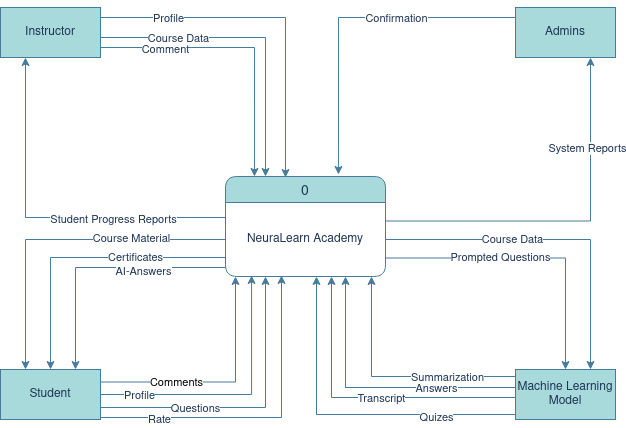
\includegraphics[max height=\textheight,max width=\textwidth]{figures/Context-Diagram.png}
	\caption{Context Diagram}
\end{figure}

\newpage


\section{Data Flow Diagram}
\begin{figure}[h!]
	\centering
	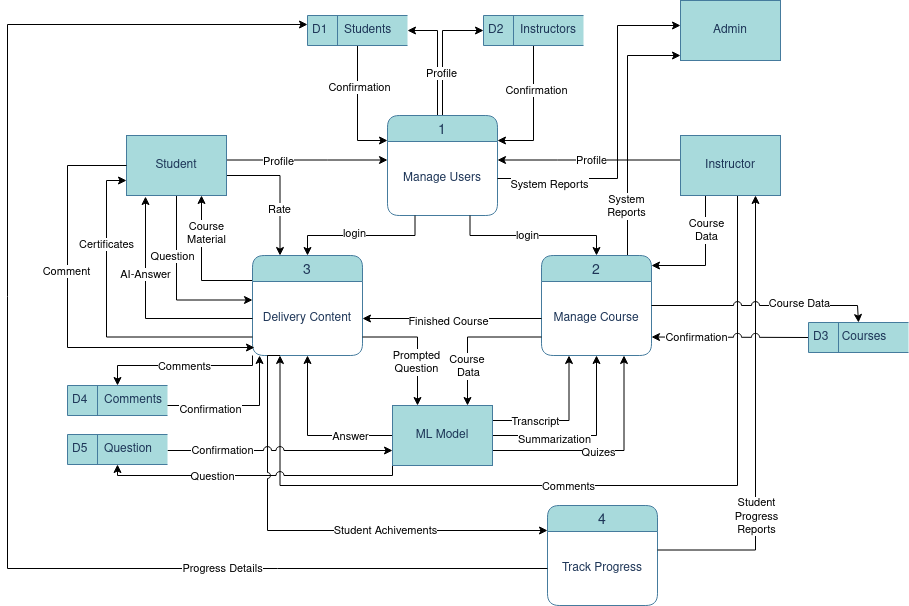
\includegraphics[max height=\textheight,max width=\textwidth]{figures/DFD.png}
	\caption{Data flow Diagram}
\end{figure}

\newpage

\section{Sequence Diagram}
\begin{figure}[h!]
	\centering
	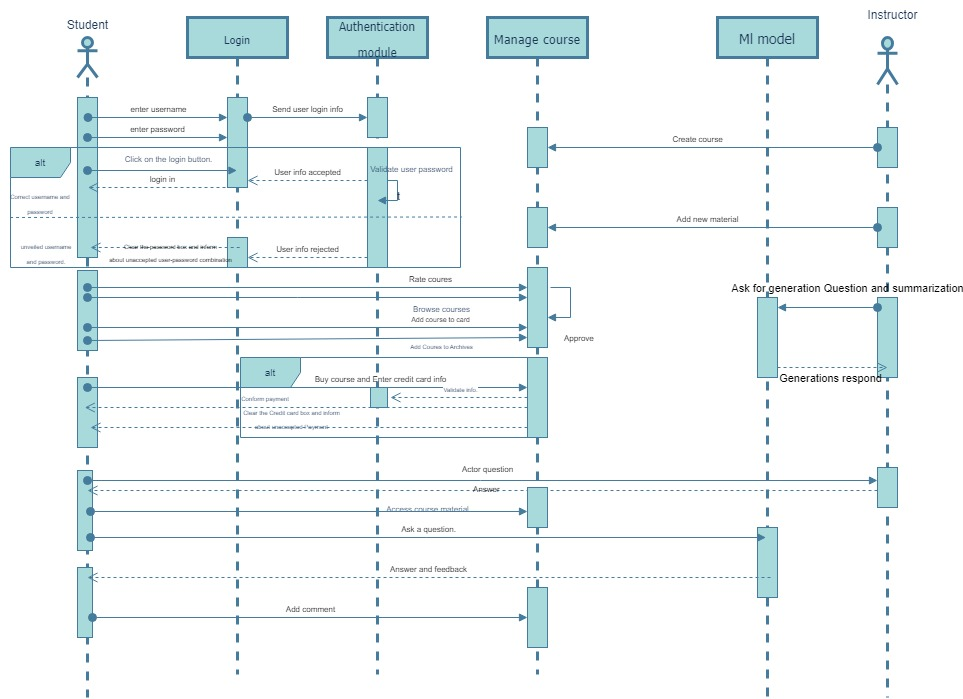
\includegraphics[max height=\textheight,max width=\textwidth]{figures/sequence.jpeg}
	\caption{Sequence Diagram}
\end{figure}

\begin{figure}[h!]
	\centering
	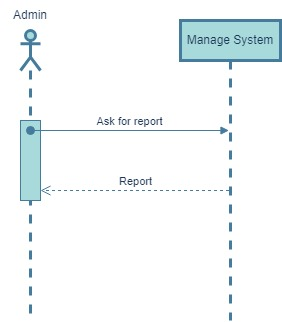
\includegraphics[width=0.40\textwidth]{figures/sequence-admin.jpeg}
	\caption{Sequence Diagram}
\end{figure}
\include{chapters/chapter4}


\end{document}
